\section{Experimentos}

A princípio foram testados variações dos parâmetros de \textit{crossover} e \textit{mutação} mantendo constante outros parâmetros. Os erros gerados no gráfico é a média da média da fitness dos indivíduos por geração em 15 instâncias de testes.

Nos gráficos, o último erro médio da geração 50 é a base de dados de teste. Percebe-se que este erro quase sempre está acima do erro do treinamento pela maldição do \textit{overfitting}.

\subsection{Crossover}

Não se percebe um impacto grande na convergência, pois depende da variabilidade da população inicial para o cruzamento encontrar novos indivíduos que contenham fitness melhores. Por exemplo, se a base de dados tiver um comportamento senoidal e nenhum indivíduo tiver uma sub-árvore que contenha seno ou cosseno. Nenhum cruzamento gerará um nó trigonométrico que diminuirá o erro.

\begin{figure}[H]
  \centering
  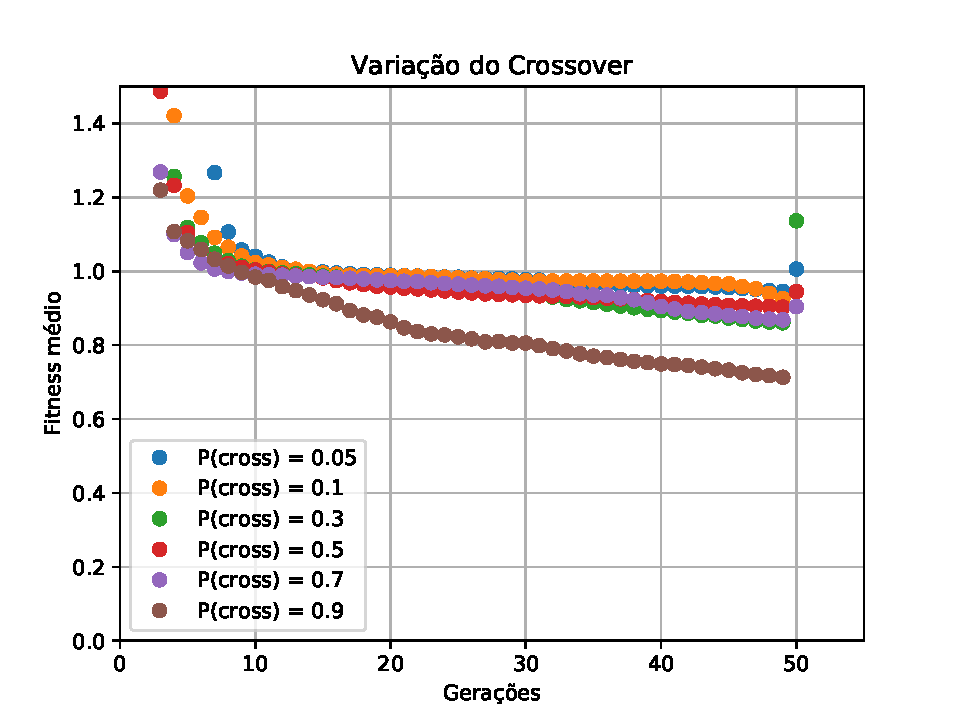
\includegraphics[width=0.5\textwidth]{pdf/varcrossover.pdf}
  \label{fig:varcross}
\end{figure}

\subsection{Mutação}

Na mutação percebemos que a convergência possui maior efeito, pois a mutação torna-se maior a variabilidade da população que probabilisticamente possui chances de algum nó gerado melhorar a fitness no treinamento.

\begin{figure}[H]
  \centering
  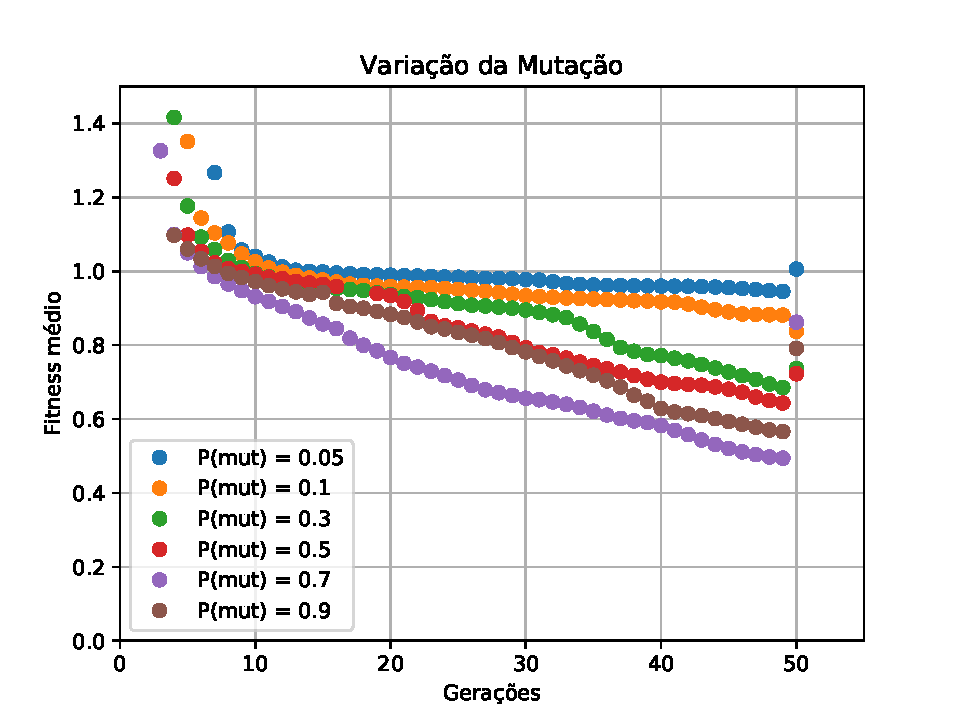
\includegraphics[width=0.5\textwidth]{pdf/varmutation.pdf}
  \label{fig:varmut}
\end{figure}

\subsection{Torneio}

O torneio percebe-se que possui uma maior pressão a convergência, mas em contra-partida diminui a variabilidade, pois em vários torneios o melhor indivíduo da população pode ser escolhido várias vezes.

\begin{figure}[H]
  \centering
  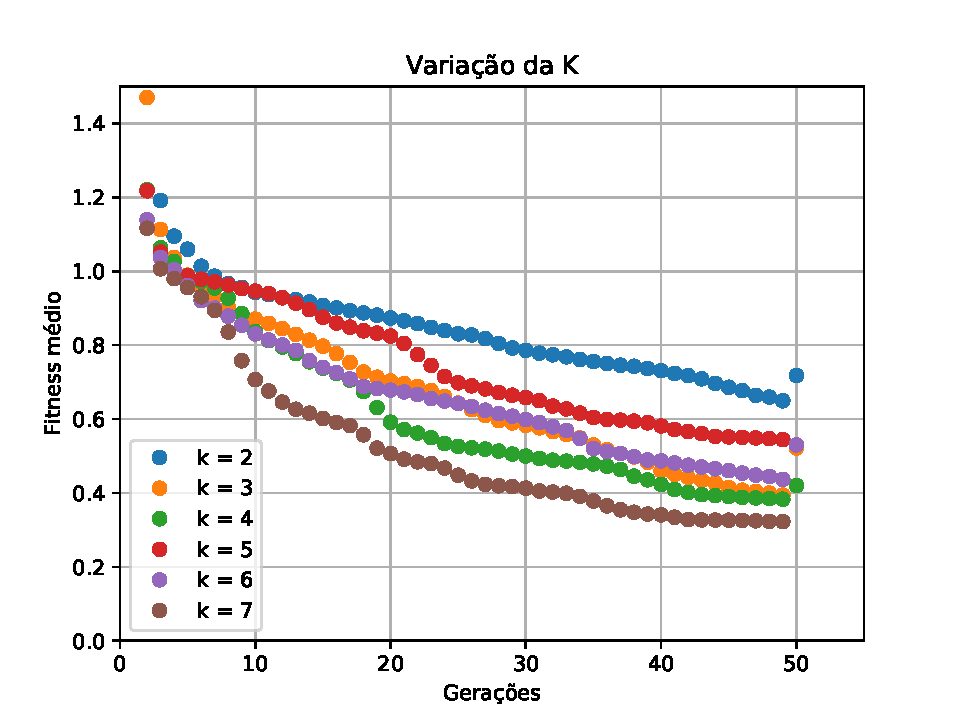
\includegraphics[width=0.5\textwidth]{pdf/varK.pdf}
  \label{fig:vark}
\end{figure}

\subsection{População}

A variação da quantidade da população impacta na variabilidade que ocasiona na probabilidade de gerar novos invivíduos diferentes. Com a convergência, observa-se que após a convergência não há mais variabilidade e a fitness e tende a permanecer constante pois não há nenhum método de \textit{niching}.

\begin{figure}[H]
  \centering
  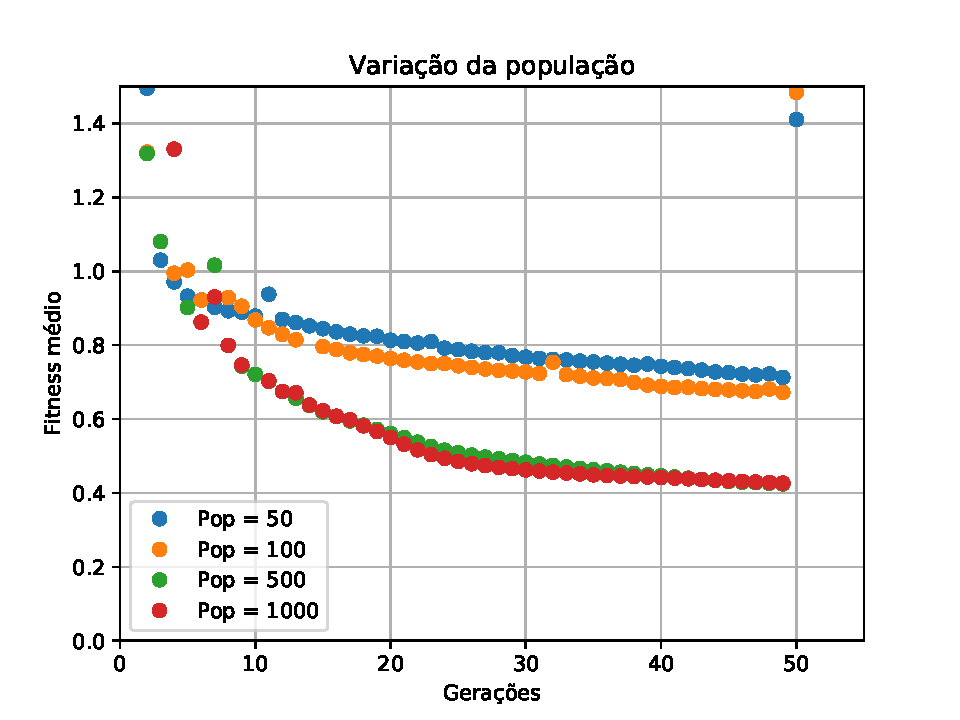
\includegraphics[width=0.5\textwidth]{pdf/populations.pdf}
  \label{fig:varpop}
\end{figure}




% • Escolher o tamanho da popula ̧c ̃ao e o nu ́mero de gerac ̧ ̃oes apropriados. O tamanho da popula ̧c ̃ao pode ser testado, por exemplo, utilizando 50, 100, 500 indiv ́ıduos. O nu ́mero de gera ̧c ̃oes pode tamb ́em ser escolhido usando esses mesmos nu ́meros. Mas como saber se o escolhido  ́e o mais apropriado? Vocˆe pode avaliar como o aumento no nu ́mero da popula ̧c ̃ao ou de gerac ̧ ̃oes melhora a soluc ̧ ̃ao encontrada (em termos do erro gerado), se a popula ̧c ̃ao converge, etc.
% • Testar duas configura ̧c ̃oes de parˆametros para cruzamento e muta ̧c ̃ao. Na primeira, a probabilidade de cruzamento (pc) deve ser alta (por exemplo, 0.9), e a probabilidade de muta ̧c ̃ao (pm) deve ser baixa (por exemplo, 0.05). Na segunda, pc deve ser mais baixa (por exemplo, 0.6) e pm mais alta (por exemplo, 0.3). Para ambas as configura ̧c ̃oes, deve-se avaliar o efeito do cruzamento e da muta ̧c ̃ao na evolu ̧c ̃ao, isto  ́e, em quantos casos esses operadores contribuem positivamente (os filhos gerados s ̃ao melhores que os pais) ou negativamente para a evolu ̧c ̃ao? A partir desse estudo inicial, que valores finais vocˆe proporia?
% • Analisar as mudan ̧cas ocorridas quando o tamanho do torneio aumenta de 2 para 5 ou 3 para 7, dependendo do tamanho inicial da popula ̧c ̃ao.
% • Analisar o impacto de usar somente operadores elitistas.
% • Existe uma forma simples de medir bloating no seu algoritmo?
